\documentclass[12pt]{article}
\usepackage{graphicx}
\usepackage{fullpage}
\usepackage{verbatim}
\usepackage{caption}
\usepackage{float}
\usepackage[nottoc]{tocbibind} 
\usepackage{appendix}
\usepackage{titlesec}
\usepackage{tikz}
\usepackage{listings}
\usepackage{hyperref}
\hypersetup{
    colorlinks=true,
    linkcolor=blue,
    filecolor=magenta,      
    urlcolor=blue,
}
\usepackage[utf8]{inputenc}
\urlstyle{same}
\usetikzlibrary{shapes,arrows}
\titleformat{\chapter}[display]
  {\normalfont\bfseries}{}{0pt}{\Large}
  \usepackage[T1]{fontenc}
\usepackage[utf8]{inputenc}

  


\begin{document}
  \begin{titlepage}
    \begin{center}
      \begin{Large}
      \textbf{ Assignment- 12\\
       \vspace*{0.5cm}
       ELP - 718 Telecom Software Laboratory\\
       \vspace{1cm}
       Ch Krishna Chaitanya\\
       2019JTM2674\\
       2019-21\\}
      \end{Large}
       \vspace{1cm}
      {\Large  A report on Behavioural Modelling in VHDL}
       \vfill
       \begin{figure}[h!]
          \centering
          
\includegraphics{iitdelhi.png}
       \end{figure}
       \vfill
      \begin{Large}
      \textbf{ Bharti School of \\
       Telecommunication Technology and Management\\
       IIT Delhi\\
       India\\
      }\end{Large}
       \medskip
       \today
    \end{center}
    \vfill
  \end{titlepage}
  
  \tableofcontents
  
  \clearpage
  \section*{Objective Statement}
   To test our understanding and implementation of digital logic in VHDL using Vivado simulator.

  \section{Problem Statement -1}
 To model a hardware that detects pattern '10110101' in input bit stream.
  
  \subsection{Algorithm and Implementation}
  \begin{itemize}
  \item Create Entity with required input ports and output ports.
  \item Draw a state diagram using Moore state machine
  \item Implement the logic in Vivado
  \item Write a test bench with required inputs
  \item Run simulation and observe output
  \end{itemize}
  \newpage
   \subsection{State Diagram}
   \begin{figure}[h!]
   \centering
   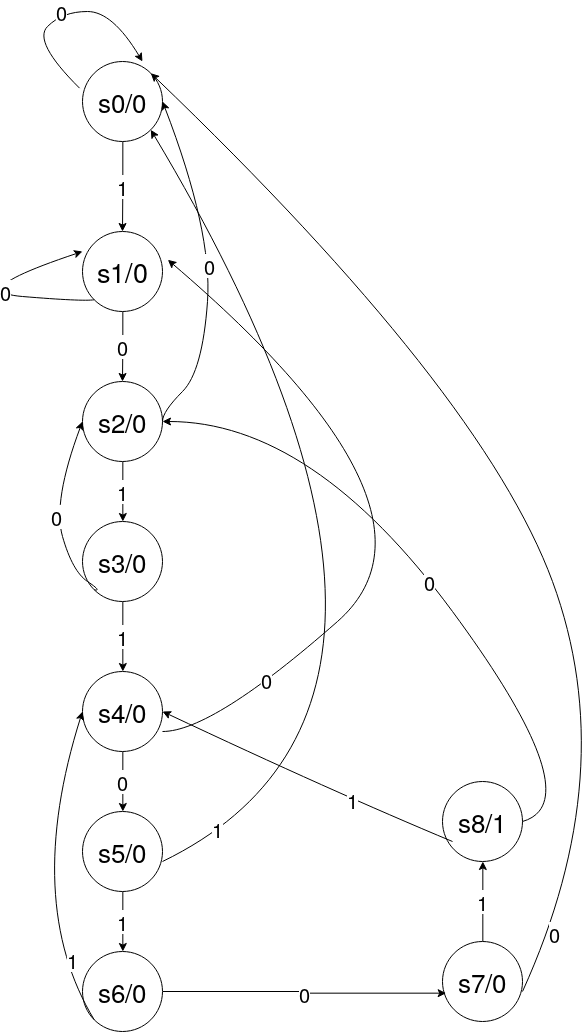
\includegraphics[width=80mm]{Image1.png}
   \caption{State Diagram}
    \label{fig:State Diagram}
   \end{figure}
  
  \subsection{Flowchart}
    % Define block styles
  \tikzstyle{decision} = [diamond, draw, fill=blue!20, 
    text width=4.5em, text badly centered, node distance=3cm, inner sep=0pt]
\tikzstyle{block} = [rectangle, draw, fill=blue!20, 
    text width=6em, text centered, rounded corners, minimum height=4.5em,node distance=2.2cm]
\tikzstyle{line} = [draw, -latex']
\tikzstyle{cloud} = [draw, ellipse,fill=red!20, node distance=3cm,
    minimum height=3em]
  \begin{center}    
\begin{tikzpicture}[node distance = 2cm, auto]
    % Place nodes
    
    \node [cloud] (init) {start};
    \node [block, below of=init] (First) {Create Entity};
    \node [block, below of=First] (Second) {Draw state diagram};
    \node [block, below of=Second] (Third) {Write VHDL code};
    \node [block, below of=Third] (Seventh) {Write test bench};
    \node [block, below of=Seventh] (Fourth) {Run Simulation};
    \node [block, below of=Fourth] (Fifth) {Observe Output};
    \node [cloud, below of=Fifth] (Sixth) {Stop};
 
    
    
    % Draw edges
    \path [line] (init) -- (First);
    \path [line] (First) -- (Second);
    \path [line] (Second) -- (Third);
     \path [line] (Third) -- (Seventh);
     \path [line] (Seventh) -- (Fourth);
    \path [line] (Fourth) -- (Fifth);
    \path [line] (Fifth) -- (Sixth);
  
   
    
\end{tikzpicture}
\end{center}
\newpage
\subsection{Inference}
Afetr implementing both mealay and moore models, following things can be observed:
\begin{itemize}
\item Number of states in Mealy is one more than in Moore.
\item Output in mealy depends on present state and input whereas in Moore it depends only on present state.
\item Output in Mealy comes a clock cycle prior, compared to Moore.
\end{itemize}
  \subsection{Screenshots}
  \subsubsection{Simulation} 
	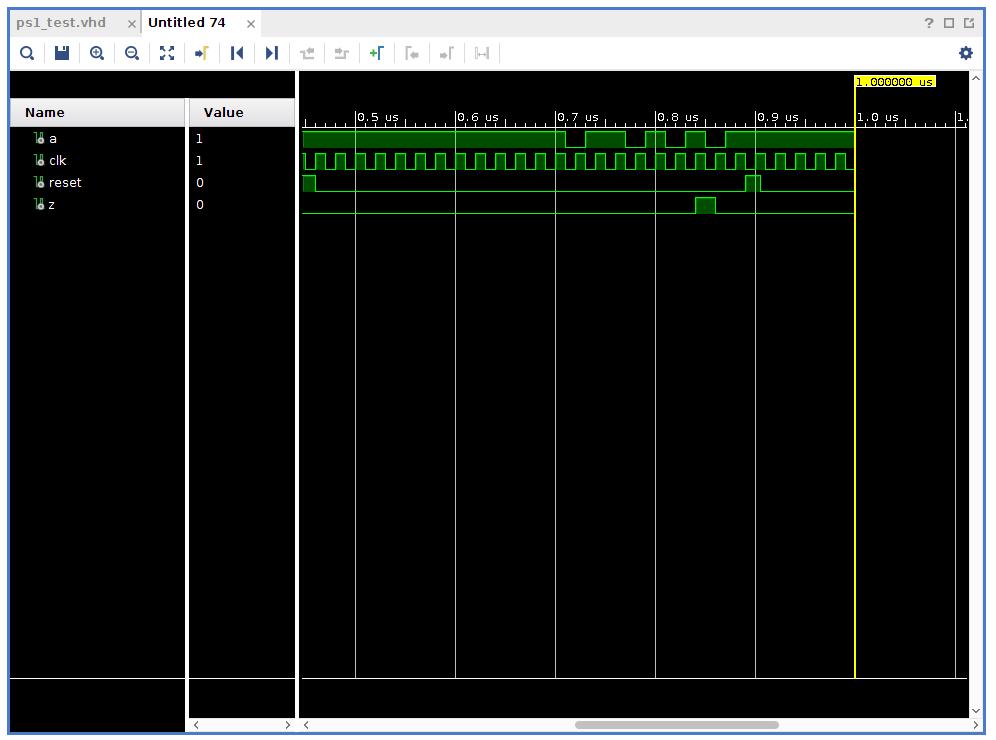
\includegraphics[width=\linewidth]{lab10_ps1b.png}
	\subsubsection{Schematic} 
	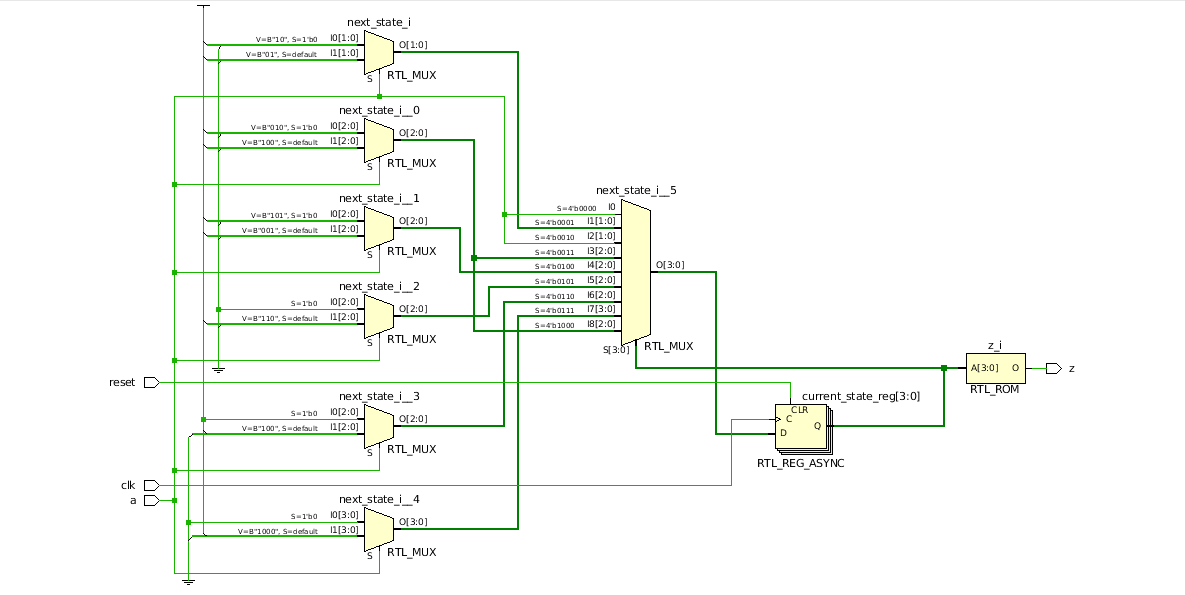
\includegraphics[width=\linewidth]{lab10_ps1.png}
\newpage
  \section{ProblemStatement-2}
  \subsection{ProblemSatement}
    To write VHDL code for frequency divider that divides input frequency by 5.



  \subsection{Algorithm}
  \begin{itemize}
  \item Create Entity with required input ports and output ports.
  \item Writ logic in VHDL that divides frequency by 5.
  \item Implement the logic in Vivado
  \item Write a test bench with clock and reset
  \item Generate output clock using testbench
  \item Run simulation and observe output
  \end{itemize}
   \subsection{Flowchart}
    % Define block styles
  \tikzstyle{decision} = [diamond, draw, fill=blue!20, 
    text width=4.5em, text badly centered, node distance=3cm, inner sep=0pt]
\tikzstyle{block} = [rectangle, draw, fill=blue!20, 
    text width=6em, text centered, rounded corners, minimum height=4.5em,node distance=2.2cm]
\tikzstyle{line} = [draw, -latex']
\tikzstyle{cloud} = [draw, ellipse,fill=red!20, node distance=3cm,
    minimum height=3em]
  \begin{center}    
\begin{tikzpicture}[node distance = 2cm, auto]
    % Place nodes
    
     \node [cloud] (init) {start};
    \node [block, below of=init] (First) {Create Entity};
    \node [block, below of=First] (Second) {Implement frequency divider};
    \node [block, below of=Second] (Third) {Writ a test bench};
    \node [block, below of=Third] (Fourth) {Run Simulation};
    \node [block, below of=Fourth] (Fifth) {Observe Output};
    \node [cloud, below of=Fifth] (Sixth) {Stop};
    
    
    % Draw edges
    \path [line] (init) -- (First);
    \path [line] (First) -- (Second);
    \path [line] (Second) -- (Third);
     \path [line] (Third) -- (Fourth);
    \path [line] (Fourth) -- (Fifth);
    \path [line] (Fifth) -- (Sixth);
  
   
    
\end{tikzpicture}
\end{center}

\subsection{Screenshots}
\subsubsection{Simulation}
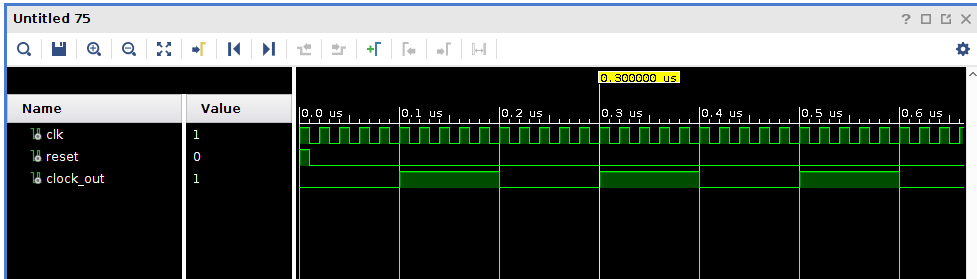
\includegraphics[width=\linewidth]{lab10_ps2a.png}

\subsubsection{Schematic}
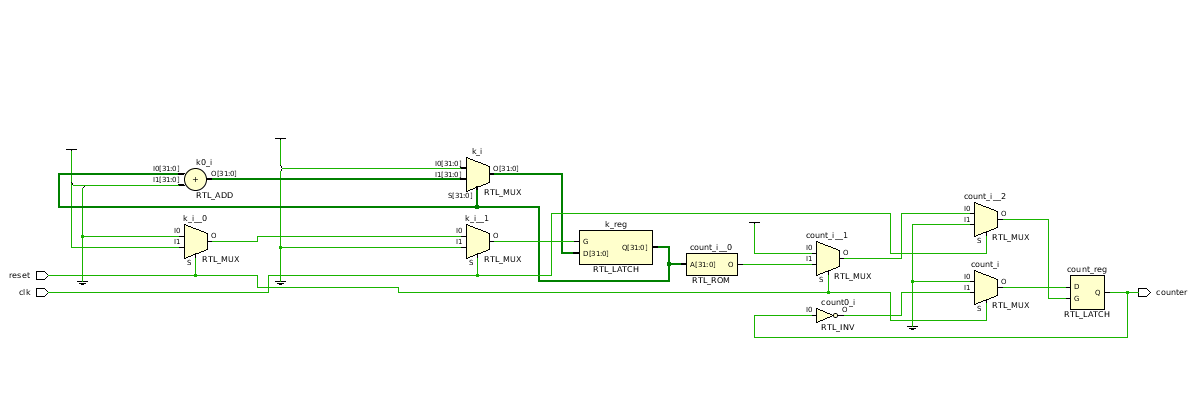
\includegraphics[width=\linewidth]{lab10_ps2b.png}

\newpage
\section{ProblemStatement-3}
 To model and simulate 15bit digital comparator with given requirements.
  
  \subsection{Algorithm}
  \begin{itemize}
  \item Create Entity with required input ports and output ports.
  \item Writ logic that implements magnitude comparator
  \item Implement the logic in Vivado
  \item Write a test bench with required inputs
  \item Run simulation and observe output
  \end{itemize}
 
   \subsection{Flowchart}
    % Define block styles
  \tikzstyle{decision} = [diamond, draw, fill=blue!20, 
    text width=4.5em, text badly centered, node distance=3cm, inner sep=0pt]
\tikzstyle{block} = [rectangle, draw, fill=blue!20, 
    text width=6em, text centered, rounded corners, minimum height=4.5em,node distance=2.2cm]
\tikzstyle{line} = [draw, -latex']
\tikzstyle{cloud} = [draw, ellipse,fill=red!20, node distance=3cm,
    minimum height=3em]
  \begin{center}    
\begin{tikzpicture}[node distance = 2cm, auto]
    % Place nodes
    
    \node [cloud] (init) {start};
    \node [block, below of=init] (First) {Create Entity};
    \node [block, below of=First] (Second) {Implement magnitude comparator};
    \node [block, below of=Second] (Third) {Writ a test bench};
    \node [block, below of=Third] (Fourth) {Run Simulation};
    \node [block, below of=Fourth] (Fifth) {Observe Output};
    \node [cloud, below of=Fifth] (Sixth) {Stop};
 
    
    
    % Draw edges
    \path [line] (init) -- (First);
    \path [line] (First) -- (Second);
    \path [line] (Second) -- (Third);
     \path [line] (Third) -- (Fourth);
    \path [line] (Fourth) -- (Fifth);
    \path [line] (Fifth) -- (Sixth);
  
   
    
\end{tikzpicture}
\end{center}
  \subsection{Screenshots}
\subsubsection{Simulation}
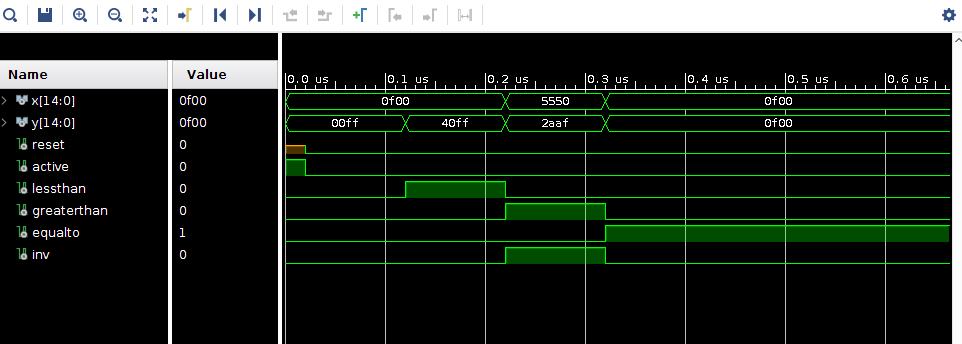
\includegraphics[width=\linewidth]{lab10_ps3a.png}

\subsubsection{Schematic}
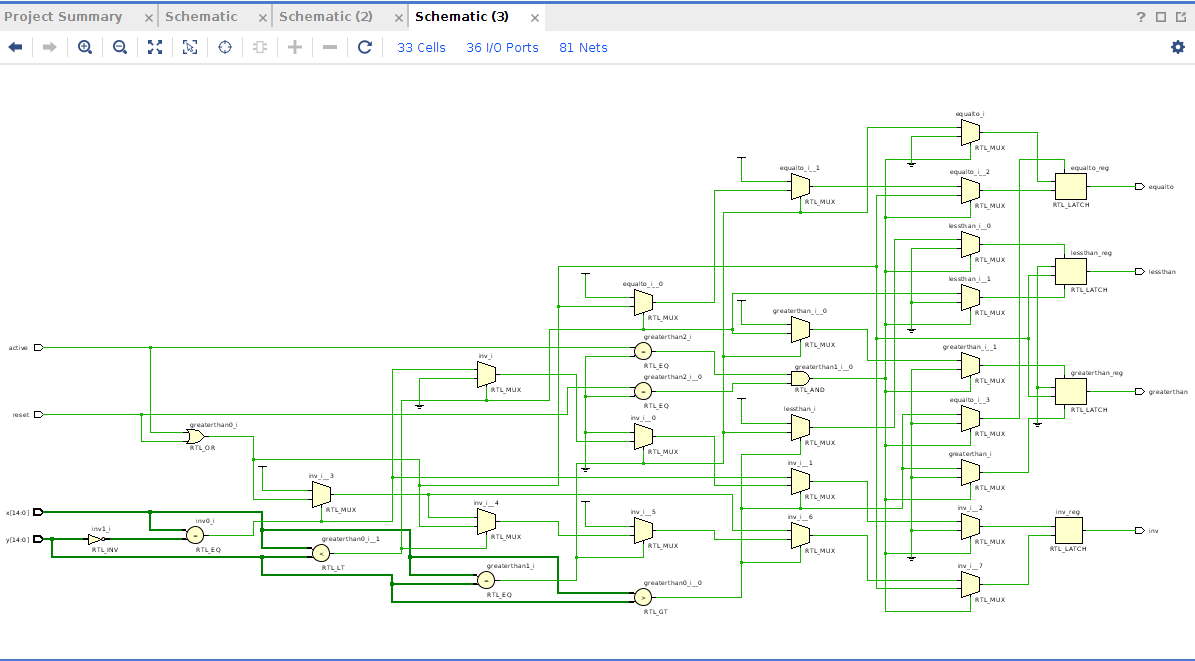
\includegraphics[width=\linewidth]{lab10_ps3b.png}
 \appendix
   \appendixpage
   \addappheadtotoc
  \section*{Problem 1}
  {\large \textbf{code:}}
  \verbatiminput{ps1.vhd}
  {\large \textbf{testbench:}}
  \verbatiminput{ps1_test.vhd}
  \section*{Problem 2}
  {\large \textbf{code:}}
  \verbatiminput{ps2.vhd}
  {\large \textbf{testbench:}}
  \verbatiminput{ps2_test.vhd}
  \section*{Problem 2}
  {\large \textbf{code:}}
  \verbatiminput{ps3.vhd}
  {\large \textbf{testbench:}}
  \verbatiminput{ps3_test.vhd}
  
  
\newpage
\begin{thebibliography}{11}
\bibitem{flowchart} 
Flowchart using Latex\\
Kjell Magne Fauske \\
\url{http://www.texample.net/tikz/examples/simple-flow-chart/}

\bibitem{VHDL Basics by Example}
VHDL Basics by Example \\
\url{http://esd.cs.ucr.edu/labs/tutorial/}

\bibitem{Finite State Machines}
Finite State Machines\\
\url{https://vhdlguide.readthedocs.io/en/latest/vhdl/fsm.html}

\bibitem{Git Hub}
Git Hub\\
\url{https://help.github.com/en/articles/fork-a-repo}

\bibitem{VHDL Test Bench}
VHDL Test Bench\\
\url{https://www.youtube.com/watch?v=2wMj-JmHDQQ}

\end{thebibliography}

   
   
\end{document}
